\section{R and Remote Sensing}


\begin{frame}{R and spatial data handling}

      \begin{itemize}[<+->]
	\item Import of raster data
	\item query data and plot spatial data
	\item compute vegetation indices
	\item we will use Landsat and MODIS data
	\item further functions will be taught soon after
      \end{itemize}

\end{frame}


\begin{frame}{R and Remote Sensing}
 
    the number of R packages specifically designed for spatial data analysis is increasing steadily:

	  \begin{itemize}
	    \item raster, rgdal: raster data analysis
	    \item maptools, sp: vector analysis
	    \item spatstat, GeoR: point statistics  
	    \item spgrass6: interface to GRASS
	    \item RSAGA: interface to SAGA GIS
	    \item read the respective manual pages for further information
	    \item don't hesitate to look at the command syntax!
	  \end{itemize}

    \vspace{1cm} \pause

	  \textcolor{gray}{
	  \begin{tiny}
	  \hspace{5cm}more information at:\\ 
	  \hspace{5cm} \url{http://geodacenter.asu.edu/r-spatial-projects/}\\ 
	  \hspace{5cm} \url{http://r-spatial.sourceforge.net/}\\
	  \hspace{5cm} \url{http://www.geog.uu.nl/~pebesma/wun/}\\
	  \hspace{5cm} \url{http://r-spatial.sourceforge.net/gallery/}\\
	  \end{tiny}
	  }


\end{frame}





\begin{frame}[fragile]{R Libraries}
      \framesubtitle{load libraries after installation}
 
    \begin{lstlisting}
	    library(raster)
	    library(rgdal)
    \end{lstlisting}

    only if packages are already installed: \textit{install.packages(``name'')}


\end{frame}


\begin{frame}[fragile]{Raster import}

\begin{lstlisting}
	b3 <- raster("/path_to_your_raster/raster.tif", band=3)
	b4 <- raster("/path_to_your_raster/raster.tif", band=4)

	summary(b3) #check the data
	image(b3)   #display raster
	plot(b3)
	spplot(b3)
    \end{lstlisting}
    
    
    \bigskip \pause image, plot und spplot commands are similar but have different (dis)advantages
    
\end{frame}




\begin{frame}{Some useful functions}
 
      \begin{description}
       \item[str(obj)] prompts the structure of an object (esp. useful for S4 Objects (spatial objects))
       \item[names(obj)] gives you the names within an object
       \item[head(obj)] shows the first rows of an object - good for first data integrity check
       \item[summary(obj)] provides summary statistics of your object
      \end{description}
 
\end{frame}


\begin{frame}[fragile]{NDVI calculation}

    \begin{lstlisting}
	ndvi<- (band_4 - band_3)/(band_4+band_3)
   \end{lstlisting}

\bigskip \pause

however if the data set is bigger, R provides more efficient ways to do it:

\bigskip \pause

 \begin{lstlisting}
	# we define a NDVI functions, so we don't have to write it several times
	fun_ndvi<- function(nir, red) {(nir-red) /(nir+red)} 
   \end{lstlisting}

   \bigskip \pause

 \begin{lstlisting}
	# NDVI
	ndvi<-overlay(band_4, band_3, fun=function(nir, red){(nir-red)/(nir+red)})
	#or
	ndvi<-overlay(band_4, band_3, fun=fun_ndvi)
   \end{lstlisting}

\bigskip \pause and you could combine it with an automatic export command (here: SAVI calculation):

 \begin{lstlisting}
	# SAVI computation with automatic data export
	savi<-overlay(band_4, band_3, fun=function(nir, red){(nir-red)/(nir+red + 0.5)*(1+0.5)}, filename="savi.tif", format="GTiff")
   \end{lstlisting}


\end{frame}


\begin{frame}[fragile]{first data manipulation}

If the raster data has negativ values and the NDVI does not display properly, do:

    \begin{lstlisting}
	# copy band 3
	b3.a <- b3
	
	#set all values below 0 to NA
	b3.a[b3.a < 0] <- NA
   \end{lstlisting}

   \bigskip
   
   and redo the NDVI  analysis.  \pause You might also want to modify the range of the NDVI values:

       \begin{lstlisting}
	# copy the ndvi data
	ndvi.a <- ndvi
	
	#set all values below 0 to NA
	ndvi.a[ndvi.a < 0] <- NA
	\end{lstlisting}
   
\end{frame}

% {\setbeamercolor{background canvas}{bg=black}
% \begin{frame}[plain]
%  \definecolor{african_dawn}{RGB}{174,162,118}
%     \begin{center}
%     \leftskip-3em
%     \vskip-2em
% 	\begin{overpic}
% 		[width=1.15\textwidth,clip=true,trim=0 0 0 00]{/a_full_cover_image.JPG}
% 		\put(5,55){\Huge{\textcolor{african_dawn}{\textbf{Compute and compare indices}}}}
% 		\put(5,45){\Huge{\textcolor{african_dawn}{\textbf{try also other indices e.g. MSAVI}}}}
% 		\end{overpic}
%     \end{center}
% 
% \end{frame}
% }



\section{more R functions}

{\setbeamercolor{background canvas}{bg=black}
\begin{frame}
 
\thispagestyle{empty}

    \vspace{6em}

          \leftskip-2.58em%
          \vskip-0.3em
          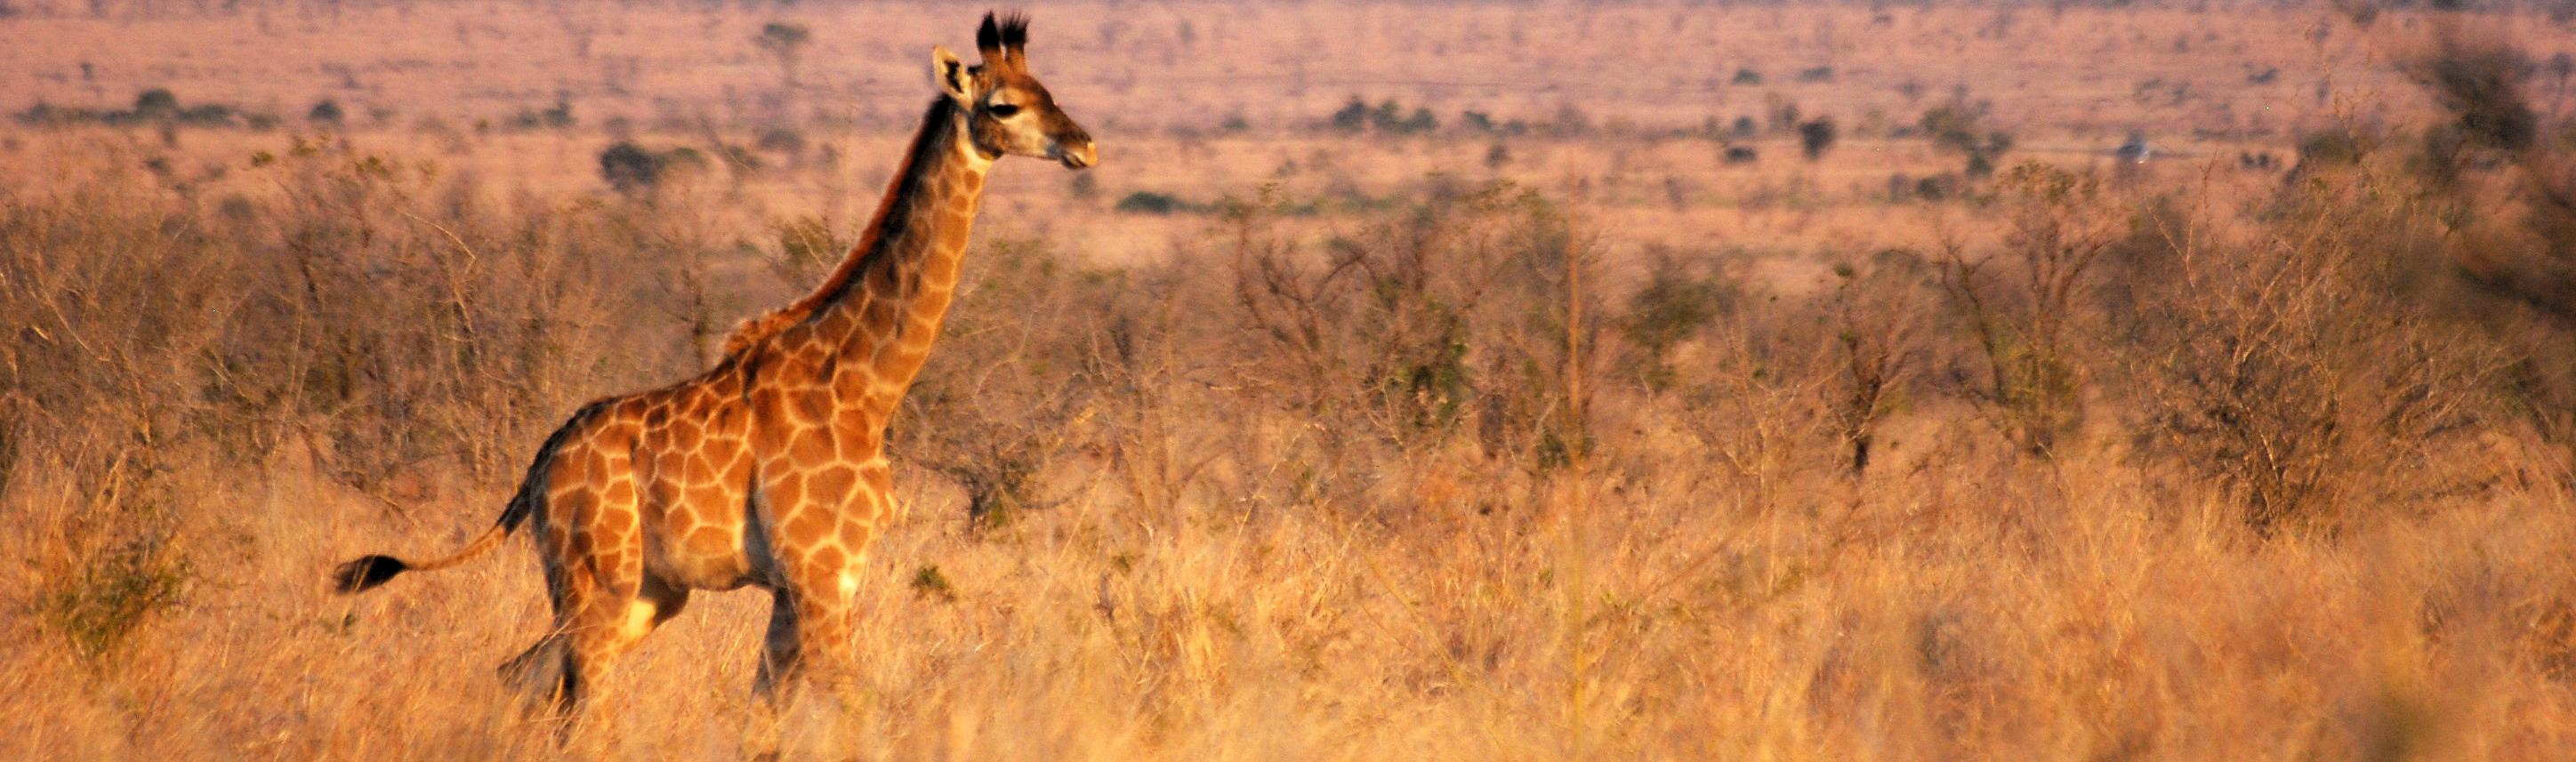
\includegraphics[width=1.28\textwidth,clip=true,trim=0 0 0 0]{giraffe_landscape_Wegmann}
            \leftskip-6.5em%
            \vskip1.5em%
  \vfill
\begin{center}\begin{LARGE}\textcolor{gray}{\textbf{More details on spatial R functions}}\end{LARGE}\end{center}
\end{frame}
}


\begin{frame}{General recommendations:}
 
      \begin{enumerate}[<+->]
	\item use all the time the scripting functions (R script including comments!)
	\item choose meaningful names: bad: my\_script.R better: ndvi\_landsat.R
	\item add meta information on top of your script: who did it, when, which R version, package versions
	\item what is the script doing, what is the result/aim
	\item and again: do execessive commenting in your script!
      \end{enumerate}

\end{frame}


\begin{frame}

    some more useful pages:
      \begin{footnotesize}
		\begin{itemize}
		  \item \url{http://rseek.org/} for general R search
		  \item \url{http://www.inside-r.org/}
		  \item \url{http://www.r-bloggers.com} 
		  \item \url{http://cran.r-project.org/web/packages/raster/vignettes/Raster.pdf}
		  \item \url{http://www.csiro.au/resources/Spatial-Point-Patterns-in-R}
		  \item \url{http://www.mo-seph.com/node/296}
		  \item \url{http://jeffreybreen.wordpress.com/2010/10/22/incremental-improvements-to-nightlights-mapping-thanks-to-r-bloggers/}
		  \item \url{http://r-nold.blogspot.de/2012/06/talking-about-elevation-one-can-also.html}
		    \item \url{http://procomun.wordpress./2012/02/20/maps_with_r_2/}
		  \item \url{http://procomun.wordpress.com/2011/06/17/raster-cmsaf-and-solar/}
		\end{itemize}
      \end{footnotesize}

\end{frame}



\begin{frame}[fragile]{Rastertypes in R}

    in R 3 different raster types exist:

      \begin{description}
       \item[Raster] one-layer raster
       \item[Brick]  multi-layer raster from one file
       \item[Stack]  Stack of 'Bricks' und 'Raster' objects from different sources
          \end{description}

          \pause \bigskip
          
\begin{lstlisting}
	# alternative to raster()
	b3 <- raster("/path_to_your_raster/raster.tif", band=3)	
	allband<- brick("/path_to_your_raster/raster.tif")
	
	#stack images or drop one
	b34<-stack(b3,allband)
	b34<-addLayer(b34, b4) 
	b5<-dropLayer(b34, 2)

	summary(b5) #check the data
    \end{lstlisting}
    
\bigskip \pause
to crop your data set use crop(), but only a rectangle will be returned, with mask() you also get an irregular shape

\end{frame}

\begin{frame}[fragile]{Raster Statistics}
      \begin{description}
	  \item[cellStats] Statistics for each layer (mean, min, max ect) 
	  \item[summary] Statistics overview based on sample of pixels (can be changed using: maxsamp)
	  \item[count] extract number of defined values
	  \item[crosstab] crosstable of 2 raster
	  \item[unique] list of all existing values
	  \item[zonal] zonal statistics for part of a raster
	  \item[quantile] compute the quantile
	\end{description}
  

    \begin{lstlisting}
	  summary(ndvi)
	  Cells:  35819702 
	  NAs  :  0 
	  Min.    0.0000
	  1st Qu. 0.3832
	  Median  0.4222
	  Mean    0.4107
	  3rd Qu. 0.4528
	  Max.    0.5748
	  summary based on a sample of 5000 cells, which is 0.0139587984288647 % of all cells 
   \end{lstlisting}

\end{frame}


\begin{frame}[fragile]{Raster query}

    \begin{lstlisting}
	b3_mod <- b3 #just generate a copy of band 3
	
	b3_mod[b3_mod > 50] <- NA #replace all values larger than 50 with NA (not available)
    \end{lstlisting}
    
    \bigskip \pause or:

    
        \begin{lstlisting}
	function1 <- function(x){x[x > 50] <- NA; return(x)} #define a function that does the same
	
	calc(b3_mod,fun=function1) #execute the function within calc()
	\end{lstlisting}

	\begin{lstlisting}
	overlay(b3_mod,fun=function1) #execute the command within overlay(); overlay() can deal with more than 1 variable
	\end{lstlisting}
	
	
	\bigskip \pause Advantage of a function? \pause you just have to define once a complex function and can easily add it everywhere in your analysis
	
\end{frame}


\begin{frame}[fragile]{Raster Logic}

     \begin{lstlisting}
	#replace value - attention: data set will be overwritten (do a copy beforehand)
	img[img>15]<-15 
	
	#List with Pixel values
	list<-img[band1==5 & band2==15] 
	
	# Raster values converted to: TRUE | FALSE
	# be aware of the capital 'W'!
	Which(band1==5 & band2!==15)

	#List with all cell-IDs which have a certain logic:
	Which(band1>122, cells=TRUE) 

   \end{lstlisting}

\end{frame}


\begin{frame}[fragile]{Raster Algebra}

    You can perform various raster manipulation tasks:
     \begin{itemize}
     \item calculates values for a raster using a formula
     \item either using calc() or overlay()
     \item computing average of all surrounding pixels
     \item either using focal() or focalFilter()
     \item compute Moran or Geary Indices (moran())
    \end{itemize}

    using:

    \begin{lstlisting}
	  formula1 <- function(x) { x * 10 }
	  rc1 <- calc(r, formula1)

	  overlay(x, fun, unstack=TRUE)

   \end{lstlisting}

      \bigskip 

      \begin{large}\textcolor{gray}{Look into the raster manual for further information and examples}\end{large}


\end{frame}

\begin{frame}[fragile]{save/export Raster }

   \begin{lstlisting}
	  # export raster - overwrite if already existent
	  writeRaster(ndvi,datatype='FLT4S', filename='NDVI.tif', format="GTiff", overwrite=TRUE)
	  
	  # assign new values to layer
	  setValues(img, values, layer)
	  
	  #set all values of first layer to 100
	  img <- setValues(img,values=100,layer=1)
	  
	  #equivalent to
	  img[[1]] <- 100
	  
	  #export image to GoogleEarth
	  KML(img, filename, col=rainbow(255), maxpixels=100000) 

   \end{lstlisting}

\end{frame}


\begin{frame}[fragile]{save/export Raster - data depth}
 \begin{lstlisting}
  dataType(img)<-value
 \end{lstlisting}

\begin{tiny}
\begin{tabular}{lll}

	Datatype definition  &minimum possible value  &maximum possible value  \\
	LOG1S  &FALSE (0)&TRUE (1)  \\
	INT1S  &-127  &127  \\
	INT1U  &0  &255  \\
	INT2S  &-32,767	32,767  \\
	INT2U  &0  &65,534  \\
	INT4S  &-2,147,483,647  &2,147,483,647  \\
	INT4U  &0  &4,294,967,296  \\
	FLT4S  &-3.4e+38  &3.4e+38  \\
	FLT8S  &-1.7e+308  &1.7e+308 \\
  
\end{tabular}
\end{tiny} 
\end{frame}


\begin{frame}[fragile]{save/export Raster file}
\begin{tiny}
\begin{tabular}{ll}

 name&long name  \\     
\hline
  raster&R-raster  \\     
  SAGA&SAGA GIS  \\     
  IDRISI&IDRISI  \\     
  BIL&Band by Line  \\     
  BSQ&Band Sequential  \\     
  BIP&Band by Pixel  \\     
  ascii&Arc ASCII  \\     
  ADRG&ARC Digitized Raster Graphics  \\     
  BMP&MS Windows Device Independent Bitmap  \\     
  BT&VTP .bt (Binary Terrain) 1.3 Format  \\     
  EHdr&ESRI .hdr Labelled  \\     
  ELAS&ELAS  \\     
  ENVI&ENVI .hdr Labelled  \\     
  ERS&ERMapper .ers Labelled  \\     
  GSBG&Golden Software Binary Grid (.grd)  \\     
  GTiff&GeoTIFF  \\     
  GTX&NOAA Vertical Datum .GTX  \\     
  HDF4Image&HDF4 Dataset  \\     
  HFA&Erdas Imagine Images (.img)  \\     
  ILWIS&ILWIS Raster Map  \\     
  INGR&Intergraph Raster  \\      
  NITF&National Imagery Transmission Format  \\     
  NTv2&NTv2 Datum Grid Shift  \\     
  PCIDSK&PCIDSK Database File  \\     
  PNM&Portable Pixmap Format (netpbm)  \\     
  RMF&Raster Matrix Format  \\     
  RST&Idrisi Raster A.1  \\     
  SAGA&SAGA GIS Binary Grid (.sdat)  \\     
  SGI&SGI Image File Format 1.0  \\     
  
\end{tabular}
\end{tiny} 
\end{frame}


 \begin{frame}{a picture}
  
  
    \begin{center}
	  \begin{overpic} 
	 [width=.5\textwidth]{giraffe_landscape_Wegmann}
	 \end{overpic}
    \end{center}
 
 
       
      \begin{textblock}{4}(16,8)
	    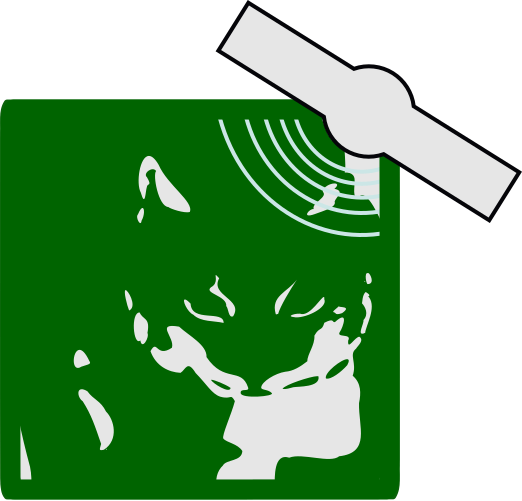
\includegraphics[width=1cm]{lynx_logo}
      \end{textblock}
  
 \end{frame}
 
